\chapter{String Gas Cosmology and the Dual-Scale Early Universe}\label{ch:cosmology}

Every chapter so far has treated the compactification radius $R$ as a parameter: a number we
choose, a point in a moduli space, a coordinate on which T-duality acts as $R\mapsto\ap/R$.
In the early universe $R$ is not a parameter but a dynamical field, and the question this
chapter asks is what T-duality does to \emph{cosmology}. The setting is string gas
cosmology\index{string gas cosmology} (SGC), the programme begun by Brandenberger and Vafa
in 1989 and reviewed by Battefeld and Watson, whose review is the source for everything
below that is not derived on the page. Three features of strings distinguish the answer
from point-particle cosmology. First, the low-energy equations of dilaton gravity have a
symmetry, scale-factor duality, that inverts the scale factor. Second, a gas of strings
contains winding modes, whose energy grows with the radius and which therefore exert
\emph{negative} pressure; a gas with equal numbers of winding and momentum modes has zero
pressure exactly at the self-dual radius, and the radius is driven there. Third, at the
self-dual radius new massless states appear, and their production as the radius passes
through that point acts as a friction that traps it. The self-dual radius of
\cref{ch:tduality}, a curiosity of the spectrum, thus becomes a dynamical attractor. We
shall also see what the argument for three large dimensions actually is and where it is
incomplete, how perturbations survive the trapping, how all this relates to the dual-scale
principle of \cref{ch:dualscale}, and exactly what the five Lean modules attached to this
chapter prove, which is much less than their names suggest.

Conventions are those of \cref{ch:circle}: mostly-plus signature, $\ap$ of dimension
length$^2$, $\ell_s=\sqrt{\ap}$. Following Battefeld--Watson (BW), $D$ is the space-time
dimension, $d=D-1$ the number of spatial dimensions in \cref{sec:cosmology:sfd} and, from
\cref{sec:cosmology:gas} on, the number of \emph{compact} directions; $\lambda_i=\ln a_i$ is
the logarithmic scale factor of direction $i$; winding numbers are $\omega$ (elsewhere $w$).

\section{Dilaton gravity and scale-factor duality}\label{sec:cosmology:sfd}

\subsection{The low-energy action}

A closed string moving in a background of its own massless fields $G_{\mu\nu}$, $B_{\mu\nu}$,
$\phi$ is described by the sigma model of \cref{ch:backgrounds}; conformal invariance at one
loop requires the vanishing of the beta functions, and those equations follow from the
space-time action \source{BW \S II, eq.~(7), ll.~343--361}
\begin{equation}\label{eq:cosmology:S0}
 S_0=\frac{1}{2\kappa_D^2}\int\dd^Dx\,\sqrt{-G}\,\ee^{-2\phi}\Bigl[R+c+4(\nabla\phi)^2-\tfrac1{12}H^2\Bigr],
 \qquad H=\dd B,
\end{equation}
where $c=0$ in the critical dimension ($D=26$ bosonic, $D=10$ super) and acts as a
cosmological constant otherwise. Two remarks on what has been dropped. The action is tree
level in $\ap$: higher-derivative terms $\ap R^2,\dots$ are neglected, which requires
curvatures small in string units. It is also tree level in the string coupling
$g_s=\ee^{\phi_0}$: the prefactor $\ee^{-2\phi}$ is the sphere's Euler characteristic, and
loops of strings would bring powers of $\ee^{2\phi}$. \source{BW \S II, ll.~362--372} Both
approximations are exactly the ones that fail near a cosmological singularity, and BW are
candid that SGC ``slowly turns on stringy effects'' rather than solving string theory in a
cosmological background. \source{BW \S III.A, ll.~549--560}

\subsection{Reduction to a mechanical system}

Take a homogeneous, anisotropic background with toroidal spatial sections and no $B$-field,
\source{BW \S II, eq.~(8), ll.~385--398}
\begin{equation}\label{eq:cosmology:ansatz}
 \dd s^2=-\dd t^2+\sum_{i=1}^{d}a_i(t)^2\,\dd x_i^2,\qquad a_i=\ee^{\lambda_i(t)},\qquad
 \phi=\phi(t),\qquad d=D-1 .
\end{equation}
The key definition is the \emph{shifted dilaton}\index{shifted dilaton}
\source{BW \S II, eq.~(9), ll.~399--404}
\begin{equation}\label{eq:cosmology:shifted}
 \varphi=2\phi-\ln V=2\phi-\sum_{i=1}^d\lambda_i ,
\end{equation}
which absorbs the volume $V=\prod a_i$ of the spatial torus into the dilaton. Let us reduce
\eqref{eq:cosmology:S0} on \eqref{eq:cosmology:ansatz}; BW state the result and we supply the
steps. For a diagonal metric $-\dd t^2+\sum\ee^{2\lambda_i}\dd x_i^2$ the Ricci scalar is
(a Christoffel computation, which we checked symbolically)
\begin{equation}\label{eq:cosmology:ricci}
 R=2\sum_i\ddot\lambda_i+\sum_i\dot\lambda_i^2+\Bigl(\sum_i\dot\lambda_i\Bigr)^2 .
\end{equation}
Write $\Lambda=\sum_i\lambda_i=\ln V$. Then $\sqrt{-G}\,\ee^{-2\phi}=\ee^{\Lambda-2\phi}=\ee^{-\varphi}$,
and with mostly-plus signature $(\nabla\phi)^2=G^{tt}\dot\phi^2=-\dot\phi^2$. The Lagrangian per unit
coordinate volume is therefore
\[
 L=\ee^{-\varphi}\Bigl[2\ddot\Lambda+\sum_i\dot\lambda_i^2+\dot\Lambda^2-4\dot\phi^2\Bigr].
\]
Now use $2\phi=\varphi+\Lambda$, so $4\dot\phi^2=\dot\varphi^2+2\dot\varphi\dot\Lambda+\dot\Lambda^2$,
and integrate the second-derivative term by parts:
$2\ee^{-\varphi}\ddot\Lambda=\frac{\dd}{\dd t}(2\ee^{-\varphi}\dot\Lambda)+2\ee^{-\varphi}\dot\varphi\dot\Lambda$.
The terms $\dot\Lambda^2$ and $2\dot\varphi\dot\Lambda$ cancel and, up to a total derivative,
\begin{equation}\label{eq:cosmology:Lmini}
 L=\ee^{-\varphi}\Bigl[\sum_{i=1}^d\dot\lambda_i^2-\dot\varphi^2\Bigr].
\end{equation}
This is the whole content of \eqref{eq:cosmology:S0} on homogeneous backgrounds: a
mechanical system with $d+1$ degrees of freedom, a kinetic term of indefinite sign (the
dilaton direction is ``time-like'', a familiar feature of gravitational minisuperspace) and
no potential. We verified with sympy that the Euler--Lagrange equations of
\eqref{eq:cosmology:Lmini} and of the unreduced Lagrangian coincide.

\subsection{Scale-factor duality}

Equation \eqref{eq:cosmology:Lmini} is manifestly invariant under
\source{BW \S II, eq.~(10), ll.~405--421}
\begin{equation}\label{eq:cosmology:sfd}
 a_i\longmapsto\frac1{a_i},\qquad \lambda_i\longmapsto-\lambda_i,\qquad \varphi\longmapsto\varphi ,
\end{equation}
for any subset of the directions $i$. This is \emph{scale-factor duality}\index{scale-factor duality}
(SFD). Since $\varphi$ is held fixed while $\ln V$ changes sign, the ordinary dilaton
transforms as $\phi\mapsto\phi-\sum_{i\in S}\lambda_i$, exactly the Buscher shift of
\cref{ch:buscher} with $R\mapsto\ap/R$. BW's reading: ``the effective field theory of dilaton
gravity for a small scale factor is equivalent to that for a large scale factor''
\source{BW \S II, ll.~424--429} --- a contracting universe and an expanding one are related by
a symmetry of the equations, a statement with no analogue in general relativity, where the
Einstein--Hilbert action reduced on \eqref{eq:cosmology:ansatz} has no such symmetry.

\begin{pitfallbox}[Scale-factor duality is not yet T-duality]
SFD is a symmetry of the \emph{massless} sector \eqref{eq:cosmology:S0} on a restricted class
of backgrounds; it knows nothing about winding strings. T-duality (\cref{ch:tduality}) is a
statement about the full string spectrum and requires the winding modes to exist. The two
agree on the spectrum of a string gas, \eqref{eq:cosmology:tdual} below, which is why one may
consistently add a string gas to dilaton gravity; but SFD alone does not say that ``small is
the same as large'' for matter.
\end{pitfallbox}

\section{A gas of strings}\label{sec:cosmology:gas}

\subsection{Assumptions}

SGC works under four stated approximations \source{BW \S III.A, ll.~517--548}: the
background fields are \emph{homogeneous} (functions of $t$ only); the evolution is
\emph{adiabatic}, so that $\ap$ corrections are negligible and each string sees a locally
constant radius; the coupling is \emph{weak}, $g_s\ll1$; and the spatial dimensions are
\emph{toroidal}, so that winding modes exist (later relaxed: orbifolds also confine). BW call
the middle two ``very restrictive from the string theory perspective''. \source{BW \S III.A,
ll.~549--560} Under them the string equation of motion reduces to the free wave equation
in conformal gauge, and the mode expansion of \cref{ch:circle} applies direction by direction.

\subsection{Energy of one string and the duality of the spectrum}

For a compact direction of radius $R$ the left- and right-moving zero-mode momenta are
$p_{L,R}=\sqrt{\ap}\,n/R\pm R\,\omega/\sqrt{\ap}$, with $n\in\Z$ the momentum and $\omega\in\Z$
the winding number. Inserting the mode expansion in the constraints gives, in the gauge
$X^0=\sqrt{\ap}E\tau$, the mass-shell condition \source{BW \S III.B, eq.~(22), ll.~680--697}
\begin{equation}\label{eq:cosmology:massshell}
 \ap E^2=\ap\vec P^2+\tfrac12(p_L^2+p_R^2)+2(N_L+N_R+a_L+a_R),
\end{equation}
where $\vec P$ is the momentum in the non-compact directions, $N_{L,R}$ are the oscillator
levels and $a_{L,R}$ the normal-ordering constants ($a_L=a_R=-1$ bosonic; heterotic
$a_L=-1$, $a_R=-\tfrac12$ in the NS sector). The second constraint gives level matching
\source{BW \S III.B, eq.~(23), ll.~716--719}
\begin{equation}\label{eq:cosmology:levelmatch}
 p_L^2-p_R^2=4n\omega=4(N_R-N_L+a_R-a_L).
\end{equation}
Since $\tfrac12(p_L^2+p_R^2)=\ap n^2/R^2+R^2\omega^2/\ap$, the bosonic case of
\eqref{eq:cosmology:massshell} with $\vec P=0$ is
$M^2=n^2/R^2+\omega^2R^2/\ap^2+(2/\ap)(N_L+N_R-2)$ with $N_R-N_L=n\omega$: precisely the mass
formula of \cref{ch:circle} (with $N=N_R$, $\tilde N=N_L$). The spectrum is invariant under
\source{BW \S III.B, eq.~(24), ll.~725--735}
\begin{equation}\label{eq:cosmology:tdual}
 \frac{R}{\sqrt{\ap}}\longmapsto\frac{\sqrt{\ap}}{R},\qquad n\longleftrightarrow\omega ,
\end{equation}
which is the T-duality of \cref{ch:tduality}. Its cosmological meaning, in BW's words, is
that ``strings at small scale factor $1/R$ behave the same as strings at large scale factor
$R$'', so that their effect on the background ``may differ greatly from that of ordinary
point particles''. \source{BW \S III.B, ll.~736--742}

\subsection{Energy density and pressure of the gas}

The $T^{00}$ component of the string stress tensor, integrated over the worldsheet, is the
energy $E$ of the string times a delta function at its position. \source{BW \S III.B,
eqs.~(25)--(27), ll.~743--800} For a gas of $N_s$ strings of each species $s$ (a species is a
choice of $n,\omega,N_L,N_R$) in spatial volume $V$, averaging the delta functions gives
\source{BW \S III.B, eqs.~(28)--(29), ll.~810--840}
\begin{equation}\label{eq:cosmology:rhop}
 \rho=\sum_s\tilde n_sE_s,\qquad \tilde n_s=\frac{N_s}{V},\qquad
 p_i=-\frac1V\frac{\partial(\rho V)}{\partial\lambda_i},
\end{equation}
the gas being treated as a non-interacting perfect fluid. The pressure formula is the
first law $\dd E=-p\,\dd V$ direction by direction: $\rho V$ is the total energy, and
$\partial/\partial\lambda_i$ is the logarithmic derivative with respect to the $i$-th
scale factor.

Consider now the two simplest gases in $d$ compact directions: pure winding strings
($\omega_m\ne0$, $n=N_L=N_R=0$) and pure momentum strings ($n_m\ne0$,
$\omega=N_L=N_R=0$), with $\vec P=0$ and the tachyonic zero-point energy removed by hand.
A string wound once around the direction $l$ has energy $R_l/\ap=\ee^{\lambda_l}/\ap$
(tension times length); a momentum mode has energy $1/R_l=\ee^{-\lambda_l}$. Absorbing the
winding and momentum numbers, and the factors of $\ap$, into the number densities
$\tilde n_w^{(l)}$, $\tilde n_m^{(l)}$: \source{BW \S III.B, eq.~(30), ll.~855--875}
\begin{equation}\label{eq:cosmology:rhowm}
 \rho_w=\sum_{l=1}^d\tilde n_w^{(l)}\ee^{\lambda_l},\qquad
 \rho_m=\sum_{l=1}^d\tilde n_m^{(l)}\ee^{-\lambda_l},\qquad
 p_w^{(l)}=-\tilde n_w^{(l)}\ee^{\lambda_l},\qquad
 p_m^{(l)}=\tilde n_m^{(l)}\ee^{-\lambda_l}.
\end{equation}
Let us derive the pressures, because a sign is at stake. The quantity held fixed when a
scale factor changes is the \emph{number} $N_w^{(l)}$ of strings, not their density. So
$\rho_wV=\sum_lN_w^{(l)}\ee^{\lambda_l}$, and
$p_w^{(l)}=-V^{-1}\partial(\rho_wV)/\partial\lambda_l=-N_w^{(l)}\ee^{\lambda_l}/V=-\tilde n_w^{(l)}\ee^{\lambda_l}$.
Likewise $p_m^{(l)}=+\tilde n_m^{(l)}\ee^{-\lambda_l}$. For an isotropic distribution
($\tilde n^{(l)}$ and $\lambda_l$ independent of $l$) the equations of state are
\source{BW \S III.B, eq.~(31), ll.~895--904}
\begin{equation}\label{eq:cosmology:eos}
 p_m=\frac1d\,\rho_m,\qquad p_w=-\frac1d\,\rho_w .
\end{equation}
Momentum modes behave as radiation filling $d$ dimensions; winding modes have negative
pressure. We checked \eqref{eq:cosmology:eos} symbolically for $d=3$.

\begin{pitfallbox}[Differentiating the density instead of the number]
If one writes $\rho_w=d\,\tilde n_w\ee^{\lambda}$ and differentiates $\rho_wV$ with $\tilde n_w$
held fixed, one obtains $p_w=-\tfrac{d+1}{d}\rho_w$ for the winding gas and
$p_m=-\tfrac{d-1}{d}\rho_m$ for the momentum gas: the momentum gas would then have negative
pressure too, which is absurd for radiation. The error is that $\tilde n=N/V$ itself depends
on $V$. Hold $N$ fixed.
\end{pitfallbox}

\begin{physicsbox}[Why winding strings pull the universe together]
A string wound around a circle is stretched: its energy is the tension $1/(2\pi\ap)$
times its length $2\pi R$. Making the circle larger costs energy, so the gas of wound
strings resists expansion\index{winding modes!negative pressure} --- that is what negative
pressure means ($\dd E=-p\,\dd V>0$ when $\dd V>0$). A momentum mode\index{Kaluza--Klein
modes} has energy $n/R$, which \emph{decreases} with $R$: it pushes outward like radiation.
In dilaton gravity\index{dilaton} the negative pressure of winding modes leads to
contraction, not to accelerated expansion as a negative-pressure fluid would in general
relativity; BW stress that this was first shown by Tseytlin and Vafa and that the
difference comes from the dilaton and from anisotropy. \source{BW \S IV.A, ll.~933--945}
\end{physicsbox}

\begin{example}[Pressure balance fixes the radius]\label{ex:cosmology:balance}
Let one compact direction of radius $b=\ee^{\nu}\sqrt{\ap}$ carry $N_w$ winding and $N_m$
momentum strings in a box of volume $V$. By \eqref{eq:cosmology:rhowm} the total pressure in
that direction is $p=(N_m\ee^{-\nu}-N_w\ee^{\nu})/V$, which vanishes when
$\ee^{2\nu}=N_m/N_w$, i.e.\ $b=\sqrt{\ap}\,(N_m/N_w)^{1/2}$. With $N_m=N_w$ the pressure-free
radius is the self-dual radius $b=\sqrt{\ap}$, and $p>0$ for $b<\sqrt{\ap}$, $p<0$ for
$b>\sqrt{\ap}$: the gas pushes the radius back toward the self-dual point from either side
(\cref{fig:cosmology:pressure}). With $N_m=4N_w$ the balance point moves to $b=2\sqrt{\ap}$,
T-dual to the balance point $b=\tfrac12\sqrt{\ap}$ of the gas with $N_m=\tfrac14N_w$, as
\eqref{eq:cosmology:tdual} requires.
\end{example}

\begin{figure}[t]
\centering
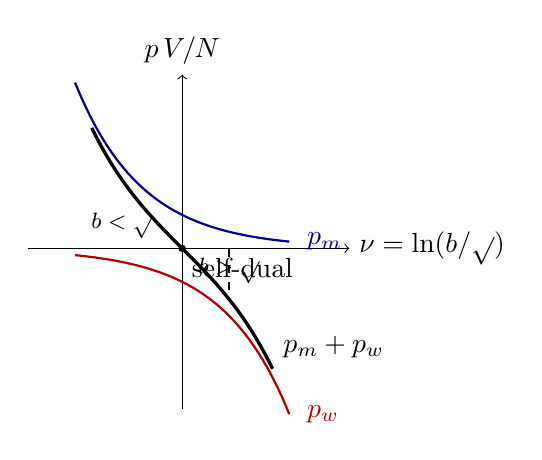
\begin{tikzpicture}[scale=0.85]
\draw[->] (-2.3,0) -- (2.5,0) node[right] {$\nu=\ln(b/\sqrt{\ap})$};
\draw[->] (0,-2.4) -- (0,2.6) node[above] {$p\,V/N$};
\draw[domain=-1.6:1.6,samples=60,smooth,thick,blue!60!black] plot (\x,{exp(-\x)/2}) node[right] {$\;p_m$};
\draw[domain=-1.6:1.6,samples=60,smooth,thick,red!70!black] plot (\x,{-exp(\x)/2}) node[right] {$\;p_w$};
\draw[domain=-1.35:1.35,samples=60,smooth,very thick] plot (\x,{(exp(-\x)-exp(\x))/2}) node[above right] {$p_m+p_w$};
\fill (0,0) circle (1.6pt) node[below right] {self-dual};
\draw[dashed] (0.7,0) -- (0.7,{(exp(-0.7)-exp(0.7))/2});
\node[below] at (0.7,0) {\footnotesize $b>\sqrt{\ap}$};
\node[above] at (-0.9,0) {\footnotesize $b<\sqrt{\ap}$};
\end{tikzpicture}
\caption{Pressure in one compact direction from a momentum gas ($p_m\propto\ee^{-\nu}$) and a
winding gas ($p_w\propto-\ee^{\nu}$) with equal numbers, \eqref{eq:cosmology:rhowm}. The sum
vanishes only at the self-dual radius and is a restoring pressure on both sides.}
\label{fig:cosmology:pressure}
\end{figure}

\begin{physicsbox}[Temperature duality and the Hagedorn transition]
Continuing time to a circle of circumference $\beta=1/T$ turns the partition function into a
thermal one, and T-duality in the time direction becomes \emph{temperature
duality}\index{temperature duality}: Giveon--Porrati--Rabinovici report that inversion of
the time-like radius $\beta$ ``was shown to be an exact symmetry to all orders in string
perturbation theory'', implying \emph{two} Hagedorn-like transitions for the heterotic
string, at $\beta_1=\sqrt2+1$ and $\beta_2=\sqrt2-1$ in string units, the second the image
of the first ($\beta_1\beta_2=1$). \source{GPR \S1, ll.~364--372} Alvarez, Alvarez-Gaum\'e and
Lozano write the free-energy form $F(\beta)=(\pi^2/\beta^2)\,F(\pi^2/\beta)$ (other
normalization of $\beta$) and add that its interpretation ``is somewhat uncertain due to the
presence of the Hagedorn temperature''. \source{AAL \S1, ll.~97--109} The Hagedorn
temperature\index{Hagedorn temperature} $T_H$, above which the exponentially growing density
of string states makes the canonical partition function diverge, is the usual starting
point of SGC (a hot gas near $T_H$); BW do not derive it and this library contains no
derivation, so the two quoted statements are \TL{} and the rest is ``standard; not checked
against a source in this book's library''.
\end{physicsbox}

\section{The Brandenberger--Vafa argument}\label{sec:cosmology:bv}

Why are three spatial dimensions large? SGC is, in BW's words, ``the only cosmological model
thus far that has attempted to explain the dimensionality of space-time dynamically''.
\source{BW \S IV.A, ll.~918--922} The argument\index{Brandenberger--Vafa mechanism} runs as
follows. \source{BW \S IV.A, ll.~922--933}
\begin{enumerate}[leftmargin=*,itemsep=1pt]
\item Start with all nine spatial dimensions compact and string-sized, filled with a hot gas
 of strings including winding modes.
\item Winding modes prevent expansion (\cref{sec:cosmology:gas}); a direction can grow only
 if its winding modes annihilate against anti-winding modes.
\item Take string interactions to be intersections of worldsheets. Two $p$-dimensional
 objects generically intersect only if $2(p+1)\le D$, i.e.\ in at most $2p+1$ spatial
 dimensions. For strings, $p=1$: two worldsheets are surfaces, which generically meet in
 points in a four-dimensional space-time and miss each other in five or more.
\item Hence winding modes can stay in equilibrium, and annihilate efficiently, in at most
 three spatial dimensions. Those three are freed to expand; the other six remain confined
 near the string scale by their winding modes.
\end{enumerate}
The dimension count in step 3 is the same one that makes two curves generically intersect
in a plane but not in space. The prediction of the argument is a $3+1+6$ split with the
three large directions radiation dominated: winding modes annihilate into unwound closed
strings, i.e.\ momentum modes, which by \eqref{eq:cosmology:eos} with $d=3$ have the
equation of state of radiation. \source{BW \S IV.C, ll.~1098--1104} Before all winding modes
have annihilated the universe \emph{loiters}\index{loitering}: the scale factor stays nearly
constant, and BW note that a loitering phase would solve the horizon problem without
inflation. \source{BW \S IV.C, ll.~1088--1100}

\begin{historybox}[The status of the argument]
BW devote a page to ``serious challenges for its quantitative realization''.
\source{BW \S IV.A, ll.~946--1001} Supergravity studies with a fixed wrapping matrix found
the anisotropic expansion but no stabilization of the internal dimensions, which merely grew
more slowly; Einstein--Boltzmann studies of a thermal brane gas found that only fine-tuned
initial conditions work: generically ``either all dimensions grow large, since the string gas
annihilated entirely, or all dimensions stay small, since the string gas froze out''. Two
reasons are given: the interaction rate is $\propto g_s^2$ and switches off as the dilaton
rolls to weak coupling; and intersection is a classical picture, whereas closed-string
exchange mediates interactions in any dimension, diluted only by $F\sim r^{-(D-2)}$. BW
conclude that ``compactification of all or none of the dimensions is the most probable
configuration'' under present knowledge, and that the argument ``is not quintessential to
string gas cosmology'': the rest of the programme \emph{assumes} the $3+6$ split as an
initial condition. \source{BW \S I, ll.~171--174; \S IV.A, ll.~985--1001} All of this is \TL{},
a report of the literature as of 2005; the dimensionality question is open.
\end{historybox}

\section{Cosmological equations with a string gas}\label{sec:cosmology:dynamics}

\subsection{The equations of motion}

Anticipating the $3+1+6$ split, take \source{BW \S IV.B, eqs.~(33)--(34), ll.~1004--1011}
\begin{equation}\label{eq:cosmology:ansatz36}
 \dd s^2=-\dd t^2+\ee^{2\lambda(t)}\dd\vec x^{\,2}+\ee^{2\nu(t)}\dd\vec y^{\,2},\qquad
 H_3=h\,\dd x^1\wedge\dd x^2\wedge\dd x^3,\qquad \phi=\phi(t),
\end{equation}
with three large directions $\vec x$, six compact ones $\vec y$ of radius
$b=\ee^{\nu}\sqrt{\ap}$ (the \emph{radion}\index{radion}), and a constant flux $h$ allowed by
the symmetry. The string gas enters the field equations through its averaged stress tensor
$T^\mu{}_\nu=\diag(-\rho,p_1,\dots,p_9)$. In terms of the total energy $E=\rho V$, the scaled
pressures $P_i=p_iV$ and the shifted dilaton $\varphi$, BW write the system as
\source{BW \S IV.B, eqs.~(38)--(41), ll.~1050--1071}
\begin{align}
 c-3\dot\lambda^2-6\dot\nu^2+\dot\varphi^2-\tfrac12h^2\ee^{-6\lambda}&=\ee^{\varphi}E,
 \label{eq:cosmology:constraint}\\
 \ddot\lambda-\dot\varphi\dot\lambda-\tfrac12h^2\ee^{-6\lambda}&=\tfrac12\ee^{\varphi}P_3,
 \label{eq:cosmology:lambdaeq}\\
 \ddot\nu-\dot\varphi\dot\nu&=\tfrac12\ee^{\varphi}P_6,
 \label{eq:cosmology:nueq}\\
 \ddot\varphi-3\dot\lambda^2-6\dot\nu^2&=\tfrac12\ee^{\varphi}E,
 \label{eq:cosmology:phieq}
\end{align}
with the conservation law $\dot E+3\dot\lambda P_3+6\dot\nu P_6=0$.
\source{BW \S IV.B, eq.~(42), ll.~1072--1079} Here $16\pi G_{10}$ has been absorbed into the
units of $E$ and $P$.

These equations can be derived in a few lines from \eqref{eq:cosmology:Lmini}, which is
instructive because it shows where each term comes from. Set $h=c=0$, put
$\lambda_{1,2,3}=\lambda$, $\lambda_{4,\dots,9}=\nu$, restore a lapse $N(t)$ (so that
$\dd t\to N\dd t$ and the kinetic term acquires a factor $1/N$), and add the matter energy
as $-NE(\lambda,\nu)$:
\begin{equation}\label{eq:cosmology:Llapse}
 L=\frac{\ee^{-\varphi}}{N}\bigl(3\dot\lambda^2+6\dot\nu^2-\dot\varphi^2\bigr)-N\,E(\lambda,\nu).
\end{equation}
The dependence of $E$ on $\lambda,\nu$ is what produces pressure: by
\eqref{eq:cosmology:rhop}, $\partial E/\partial\lambda_i=-P_i$, so with three equal
directions $\partial E/\partial\lambda=-3P_3$ and $\partial E/\partial\nu=-6P_6$. Varying $N$
and then setting $N=1$ gives the constraint \eqref{eq:cosmology:constraint}. Varying
$\lambda$: $\frac{\dd}{\dd t}(6\ee^{-\varphi}\dot\lambda)=-\partial E/\partial\lambda=3P_3$, i.e.\
$6\ee^{-\varphi}(\ddot\lambda-\dot\varphi\dot\lambda)=3P_3$, which is \eqref{eq:cosmology:lambdaeq};
$\nu$ gives \eqref{eq:cosmology:nueq} in the same way. Varying $\varphi$:
$\frac{\dd}{\dd t}(-2\ee^{-\varphi}\dot\varphi)=-\ee^{-\varphi}(3\dot\lambda^2+6\dot\nu^2-\dot\varphi^2)$,
i.e.\ $2\ddot\varphi=\dot\varphi^2+3\dot\lambda^2+6\dot\nu^2$; eliminating $\dot\varphi^2$ with the
constraint yields \eqref{eq:cosmology:phieq}. The conservation law is the chain rule
$\dot E=\partial_\lambda E\,\dot\lambda+\partial_\nu E\,\dot\nu$. We confirmed all four
equations with sympy from \eqref{eq:cosmology:Llapse}.

Two structural facts follow. First, $\ee^{\varphi}=\ee^{2\phi}/V=g_s^2/V$: the string gas
couples to the geometry with strength $g_s^2$, as matter should at one loop. Second, the
dilaton is sourced by the \emph{trace} of the stress tensor, so ``the dilaton can only
evolve if matter is not conformal''; a string gas is not conformal, ``and it is this
important observation that makes string cosmology (dilaton gravity) very different from
ordinary cosmology''. \source{BW \S IV.B, ll.~1030--1040}

\subsection{Stabilization of the radion at the self-dual radius}

Fill the six compact directions with equal numbers of winding and momentum strings and let
the three large ones expand. Watson and Brandenberger found that the radion then
\emph{oscillates about the self-dual radius}, driven by the competing pressures of
\cref{ex:cosmology:balance}, and that the oscillations are damped provided the dilaton runs
to weak coupling. \source{BW \S IV.C, ll.~1105--1135} Let us see this in
\eqref{eq:cosmology:nueq}.

\begin{example}[Small oscillations of the radion]\label{ex:cosmology:radion}
With $N_w=N_m=N$ strings per compact direction, $P_6=N(\ee^{-\nu}-\ee^{\nu})\approx-2N\nu$ for
small $\nu$, and \eqref{eq:cosmology:nueq} becomes
\begin{equation}\label{eq:cosmology:radionosc}
 \ddot\nu-\dot\varphi\,\dot\nu+\ee^{\varphi}N\,\nu=0 .
\end{equation}
This is a damped oscillator with frequency $\Omega^2=\ee^{\varphi}N=g_s^2N/V$ and friction
coefficient $-\dot\varphi$. Running to weak coupling means $\dot\phi<0$, and with $V$
growing, $\dot\varphi=2\dot\phi-\dot{\ln V}<0$ as well, so the friction term has the right
sign: the dilaton damps the radion, which is BW's Figure~1 in a formula. In string units,
with $g_s=0.1$ and one string of each type per unit string volume, $\Omega=0.1/\sqrt{\ap}$
and the period is $2\pi/\Omega\approx63\sqrt{\ap}$; the frequency falls with the coupling,
and the restoring force disappears if the gas is diluted away --- the seed of the difficulty
discussed next.
\end{example}

\subsection{The Einstein-frame objection}

The stability just found is a string-frame statement. At late times the physically
meaningful frame is the four-dimensional Einstein frame, in which Newton's constant is fixed;
a rolling dilaton would make $G_N$ time dependent, which fifth-force experiments exclude.
\source{BW \S IV.D, ll.~1191--1200} Rewriting the ten-dimensional string-frame metric in
Einstein frame, \source{BW \S IV.D, eq.~(43), ll.~1201--1204}
\begin{equation}\label{eq:cosmology:einsteinframe}
 \dd s_E^2=-\dd t_E^2+\ee^{\phi/2}a^2(t)\,\dd\vec x^{\,2}+\ee^{\phi/2}b^2(t)\,\dd\vec y^{\,2},
 \qquad \dd t_E^2=\ee^{\phi/2}\dd t_s^2 ,
\end{equation}
shows the problem at a glance: even if $b(t)$ is frozen, the Einstein-frame radius
$\ee^{\phi/4}b$ keeps evolving as long as the dilaton does. BW insist that ``the two frames
are physically equivalent, but the instability is manifest in the Einstein frame''
\source{BW \S IV.D, ll.~1212--1222}: a conformal rescaling changes no prediction, only which
variable is called ``the radius''\index{Einstein frame}\index{string frame}, so a claim of
stabilization must always say in which frame, and whether the dilaton has been fixed.

Reducing to four dimensions and canonically normalizing the dilaton and radion ($\phi$ and
$\psi$ below), the potential of a gas of $N$ objects of type $k$ wrapped on the compact
space is, in the Einstein frame and at weak coupling ($\phi\to-|\phi|$),
\source{BW \S IV.D, eqs.~(46)--(48), ll.~1270--1321}
\begin{equation}\label{eq:cosmology:Vwind}
 V_E^{(4)}=\mu\tilde n\,\ee^{\phi}\,b^{\,k-d/2}
 =\mu\tilde n\,\ee^{-|\phi|}\exp\Bigl(\frac{2k-d}{2\sqrt{2d}}\,\psi\Bigr),
\end{equation}
where $k=1$ for a wound string, $k=-1$ for a string with momentum, $k=2$ for a wrapped
2-brane, and $\mu=(2\pi\sqrt{\ap})^{-4}$. The exponent of $b$ is the string-frame exponent
$k$ of the energy shifted by $-d/2$, the shift coming from the Weyl rescaling that removes
the volume factor from the four-dimensional Einstein term. A confining potential requires a
positive power, $k\ge d/2$: for winding strings ($k=1$) this holds only for $d=1$, and for
$d=6$ the exponent is $1-3=-2$, a runaway. Hence BW's conclusion: ``a gas of purely winding
strings is not enough to stabilize the extra dimensions'', and the overall $\ee^{-|\phi|}$
dilutes whatever potential there is. \source{BW \S IV.D, ll.~1322--1333}

\subsection{States that become massless at the self-dual radius}

The remedy proposed by Watson and Brandenberger is to include the string states that are
massless \emph{exactly} at the self-dual radius. For the heterotic string in its NS ground
state ($N_R=\tfrac12$, $N_L=0$), the energy and level-matching condition for a state with
momentum and winding vectors $n,\omega\in\Z^d$ on a square torus of radius $b$ are
\source{BW \S IV.D, eqs.~(49)--(51), ll.~1340--1376}
\begin{equation}\label{eq:cosmology:hetE}
 E^2=\Bigl|\frac{n}{b}+\frac{\omega b}{\ap}\Bigr|^2-\frac{4}{\ap},\qquad n\cdot\omega=1 ,
\end{equation}
which at $b=\sqrt{\ap}$ vanishes precisely when \source{BW \S IV.D, eq.~(52), ll.~1385--1392}
\begin{equation}\label{eq:cosmology:esp}
 n\cdot n+\omega\cdot\omega=2,\qquad n\cdot\omega=1 ,
\end{equation}
i.e.\ $n=\omega=\pm e_m$ for a unit vector $e_m$. Away from the self-dual radius, with
$n=\omega$ along one direction and $b$ in units of $\sqrt{\ap}$,
\source{BW \S IV.D, eq.~(54), ll.~1418--1426}
\begin{equation}\label{eq:cosmology:Eesp}
 E=\sqrt{\frac{n\cdot n}{b^2}+\omega\cdot\omega\,b^2-2n\cdot\omega}
 =\Bigl|\frac1b-b\Bigr|=2\Bigl|\sinh\Bigl(\frac{\psi}{\sqrt{2d}}\Bigr)\Bigr|,
\end{equation}
the last form for $b=\ee^{\psi/\sqrt{2d}}$, the normalization of $\psi$ implied by
\eqref{eq:cosmology:Vwind} (BW omit the absolute value). For $b=1.2\sqrt{\ap}$ the mass is
$|1/1.2-1.2|=11/30\approx0.37$
in units of $1/\sqrt{\ap}$: a state that is massless at the self-dual point is already a
third of the string scale $20\%$ away from it. Its potential in the Einstein frame,
\source{BW \S IV.D, eq.~(55), ll.~1440--1451}
\begin{equation}\label{eq:cosmology:Vesp}
 V_E^{(4)}=2\mu\tilde n\,\ee^{\phi-\frac12\sqrt{d/2}\,\psi}\Bigl|\sinh\Bigl(\frac{\psi}{\sqrt{2d}}\Bigr)\Bigr|,
\end{equation}
does have a local minimum, but it ``becomes shallow'' as the dilaton runs to weak coupling.
\source{BW \S IV.D, ll.~1452--1456} BW then raise the objection that decides the matter:
away from $b=\sqrt{\ap}$ these states are string-scale heavy and do not belong in a
low-energy effective action, and ``if we include one massive state of the string, don't we
have to include all of them?'' --- other states become light at other points of moduli
space, each an attractor, and which one traps the radion depends on initial conditions.
\source{BW \S IV.D, ll.~1457--1472}

\section{Quantum moduli trapping}\label{sec:cosmology:trapping}

The resolution BW favour is to keep only the massless fields in the action and to let the
extra states be \emph{produced} quantum mechanically when the radion passes near a point
where they become massless, an \emph{enhanced symmetry point}\index{enhanced symmetry point}
(ESP). \source{BW \S V, ll.~1490--1510} The produced particles then have masses that grow with
the distance from the ESP, and their energy density is a potential that pulls the radion
back. This is \emph{quantum moduli trapping}\index{moduli trapping}, a mechanism first
studied for D-brane moduli by Kofman et al.\ and adapted to SGC by Watson.

\subsection{The spectrum at the self-dual radius}

Take the bosonic string on $M_4\times S^1$ with radius $R$ and radion
$\sigma=\ln(R/\sqrt{\ap})$. The mass formula and level matching are
\source{BW \S V, eq.~(59), ll.~1580--1587}
\begin{equation}\label{eq:cosmology:M59}
 M^2=\frac{n^2}{R^2}+\frac{\omega^2R^2}{\ap^2}+\frac2{\ap}(N_L+N_R-2),\qquad n\omega+N_L-N_R=0 .
\end{equation}
At generic radius the massless states have $n=\omega=0$, $N_L=N_R=1$: the graviton,
$B$-field and dilaton (oscillators in the non-compact directions), the radion $\sigma$ (both
oscillators in the compact direction) and two vectors $A_\mu=\tfrac12(G_{\mu5}+B_{\mu5})$,
$\bar A_\mu=\tfrac12(G_{\mu5}-B_{\mu5})$, a $U(1)_L\times U(1)_R$ gauge theory.
\source{BW \S V, eqs.~(60)--(62), ll.~1620--1660} At $R=\sqrt{\ap}$ substitute
$N_R=N_L+n\omega$ into $\ap M^2=n^2+\omega^2+2(N_L+N_R-2)$:
\begin{equation}\label{eq:cosmology:M64}
 \ap M^2=(n+\omega)^2+4(N_L-1),\qquad n\omega+N_L-N_R=0 ,
\end{equation}
which is BW's eq.~(64). \source{BW \S V, ll.~1670--1678} Massless states need
$(n+\omega)^2=4(1-N_L)$, hence $N_L\in\{0,1\}$. For $N_L=1$: $n=-\omega$ and $N_R=1-\omega^2\ge0$
forces $\omega=0$ (the generic states) or $(n,\omega)=(\pm1,\mp1)$ with $N_R=0$. For $N_L=0$:
$n+\omega=\pm2$ and $N_R=n\omega\in\{0,1\}$, giving $(\pm2,0)$, $(0,\pm2)$ with $N_R=0$ and
$(\pm1,\pm1)$ with $N_R=1$. A computer enumeration over $|n|,|\omega|\le3$, $N_{L,R}\le2$
finds exactly these nine $(n,\omega,N_L,N_R)$ combinations (including $(0,0,1,1)$). With
the excited oscillator along the circle they are scalars, along $M_4$ vectors: four new
vectors join $A_\mu,\bar A_\mu$ to form the adjoint of $SU(2)_L\times SU(2)_R$, and eight
new scalars join $\sigma$ to form its $(\mathbf3,\mathbf3)$. \source{BW \S V, ll.~1690--1770}
This is the enhanced gauge symmetry of \cref{ch:tduality}, now a cosmological event. The
gauge coupling gives the new states masses $m_A^2\sim g^2\sigma^2$: the radion is a Higgs
field for $SU(2)\times SU(2)$, with $g$ of order one in string units.
\source{BW \S V, ll.~1780--1800}

\subsection{Production and backreaction}

Freeze the dilaton and keep only the four-dimensional metric $\ee^{2\lambda}$, the radion
$\sigma$ and one of the new vectors $A_\mu$ with the coupling \source{BW \S V, eq.~(75),
ll.~1880--1885}
\begin{equation}\label{eq:cosmology:Veff}
 V_{\rm eff}(\sigma,A)=\tfrac12(\partial_\mu A_\nu)^2-\tfrac12g^2\sigma^2A_\mu A^\mu ,
\end{equation}
so that $m^2(t)=g^2\sigma(t)^2$ is a time-dependent mass. Before production the radion is a
free field with $\rho=p$, its kinetic energy scales as $a^{-6}$, $a\sim t^{1/3}$, and
$\sigma(t)=\sigma_0+v_0t$ with $\sigma_0=0$ if the radion passes exactly through the ESP.
\source{BW \S V, eqs.~(71)--(74), ll.~1830--1852} A Fourier mode of $A$ has frequency
$\omega_k=\sqrt{k^2+g^2\sigma^2}$ and is excited when its evolution is non-adiabatic,
$\dot\omega_k/\omega_k^2\ge1$; the resulting occupation number is
\source{BW \S V, eqs.~(76)--(77), ll.~1900--1916}
\begin{equation}\label{eq:cosmology:nk}
 n_k=\exp\Bigl(-\frac{\pi(k^2+g^2\sigma_0^2)}{gv_0}\Bigr),
\end{equation}
the standard result for a mass that passes linearly through zero. Integrating,
\source{BW \S V, eq.~(78), ll.~1920--1926}
\begin{equation}\label{eq:cosmology:rhoA}
 \rho_A=\int\frac{\dd^3k}{(2\pi)^3}\,n_k\,\omega_k\approx g|\sigma(t)|\,\mathcal N,
 \qquad \mathcal N\sim(gv_0)^{3/2},
\end{equation}
because once $\sigma$ has moved on, $\omega_k\approx g|\sigma|$ for all produced modes.
Since the energy in $A$ grows linearly with $|\sigma|$, it is a potential $V=g\mathcal N|\sigma|$
with a constant restoring force of magnitude $g\mathcal N$ pointing back to the ESP, and the
radion equation becomes \source{BW \S V, eq.~(79), ll.~1930--1937}
\begin{equation}\label{eq:cosmology:trap}
 \ddot\sigma+3\dot\lambda\,\dot\sigma=-g\mathcal N(t)\,\sgn\sigma .
\end{equation}
Each passage through the ESP converts radion kinetic energy into particles, the force never
changes sign, Hubble friction $3\dot\lambda\dot\sigma$ damps what remains, and the radion
settles at $\sigma=0$: BW conclude that friction plus backreaction ``should be more than
adequate to stabilize the radion at the self dual radius''. \source{BW \S V, ll.~1940--1957}

\begin{example}[Which modes are produced]\label{ex:cosmology:modes}
With $\sigma=v_0t$ and $\sigma_0=0$, $\dot\omega_k/\omega_k^2=g^2v_0^2t/(k^2+g^2v_0^2t^2)^{3/2}$.
For fixed $k$ this is maximal at $t_*=k/(\sqrt2\,gv_0)$, where it equals
$2\sqrt3\,gv_0/(9k^2)$. The non-adiabaticity condition $\ge1$ is therefore met only for
$k^2\le(2\sqrt3/9)\,gv_0\approx0.38\,gv_0$, in agreement with the Gaussian width of
\eqref{eq:cosmology:nk}, and only during $|t|\lesssim(gv_0)^{-1/2}$. The integral of
\eqref{eq:cosmology:nk} is exactly $\mathcal N=(gv_0)^{3/2}/(8\pi^3)$ (a Gaussian integral we
evaluated with sympy), which fixes the constant in \eqref{eq:cosmology:rhoA}. For $g=1$ and a
radion velocity $v_0=10^{-2}$ in string units, $\mathcal N\approx4\times10^{-6}$ particles per
string volume are produced per crossing: trapping is efficient only when the radion arrives
fast, and Hubble friction finishes the job.
\end{example}

The dilaton is the loose end. Its stabilization would need enhanced-symmetry states whose
mass depends on $g_s$, which requires knowing the theory at all couplings; BW mention BPS
membrane bound states in M-theory as a candidate and leave the question open.
\source{BW \S V, ll.~1958--1980} Nothing in this chapter fixes the dilaton, and every
stabilization statement above is conditional on its being fixed by other means.

\section{Perturbations and superhorizon freezing}\label{sec:cosmology:perturbations}

Does the violent production of a string gas and the trapping of the radion destroy a
pre-existing spectrum of cosmological perturbations? BW report the result of Battefeld et
al.\ (2005), obtained in a five-dimensional setting with a classical gas of massless string
modes and a radiation bath, all perturbed to first order: ``long wavelength modes of the
Bardeen potentials (super horizon modes) stay approximately frozen until they re-enter the
Hubble horizon, since the transient oscillations of the radion only source equally
transient oscillations in the Bardeen potentials'', and the radion perturbation itself has
only decaying modes. A spectrum thus ``will survive the trapping of the radion in a similar
way as a spectrum survives reheating''. \source{BW \S VI.B, ll.~2263--2281} The weak point, in
BW's own words, is that no realization of inflation exists within SGC, so the spectrum
whose survival is established must be supplied from outside. \source{BW \S VI.B, ll.~2246--2262}

The standard tool for such questions, which this book's source library does not contain and
which we therefore state as ``standard; not checked against a source in this book's
library'', is the Mukhanov--Sasaki equation\index{Mukhanov--Sasaki equation}. For a single
scalar clock in a flat FRW universe, the gauge-invariant variable $v=z\,\mathcal R$ (with
$\mathcal R$ the comoving curvature perturbation and $z=a\dot\varphi_{\rm clock}/H$) obeys, in
conformal time $\eta$ and for each comoving wavenumber $k$,
\begin{equation}\label{eq:cosmology:MS}
 v_k''+\Bigl(k^2-\frac{z''}{z}\Bigr)v_k=0 ,
\end{equation}
and the scalar power spectrum is $\mathcal P_s(k)=\frac{k^3}{2\pi^2}\bigl|v_k/z\bigr|^2$.
\emph{Superhorizon freezing}\index{superhorizon freezing} is the following elementary fact.
When $k^2\ll z''/z$ the equation is $v''=(z''/z)v$, whose two solutions are $v=z$ and
$v=z\int^\eta\dd\eta'/z^2$ (check: $(z\,w)''=z''w+2z'w'+zw''$ with $w'=1/z^2$, and
$2z'/z^2+z(-2z'/z^3)=0$). For an expanding universe $z$ grows and the second solution
decays relative to the first, so $v_k/z\to C_k$, a constant: $\mathcal R$ is conserved
outside the horizon. This is the precise content of ``modes stay frozen until they
re-enter''. What Battefeld et al.\ showed is that the same holds for the Bardeen
potentials\index{Bardeen potential} in the five-dimensional string-gas model, a separate
calculation \TL{} that we have not reproduced.

\section{The dual-scale reading}\label{sec:cosmology:dualscale}

The dual-scale principle of \cref{ch:dualscale} treats $R$ and $\ap/R$ on an equal footing
through the effective scale $R+\ap/R\ge2\sqrt{\ap}$, with equality at the self-dual radius.
This chapter lets us say precisely which parts of the cosmological story that inequality
supports.
\begin{itemize}[leftmargin=*,itemsep=2pt]
\item \TA{} The inequality itself: $R+1/R\ge2$ for real $R>0$ (\cref{ch:dualscale}), and
 $R^2+1\ge2$ for naturals $R\ge1$ (\cref{ch:stabilization}). Elementary, kernel-checked,
 and about numbers. In Lean:\\
 \lean{circle\_effective\_scale\_ge\_two} (reals) and\\
 \lean{self\_dual\_is\_global\_minimum} (naturals).
\item \TL{} The self-dual radius as a cosmological attractor. That a gas with equal winding
 and momentum numbers has zero pressure at $b=\sqrt{\ap}$ (\cref{ex:cosmology:balance}),
 that the radion oscillates about that point and is damped by the running dilaton
 (\cref{ex:cosmology:radion}), and that ESP particle production traps it there
 (\cref{sec:cosmology:trapping}), are results of the SGC literature as reviewed by BW, with
 the qualifications recorded above (frame dependence, dilaton unstabilized, initial
 conditions). The energy \eqref{eq:cosmology:Eesp}, $|1/b-b|$, is the dual-scale
 combination with a minus sign; $b+1/b$ is the energy of one winding plus one momentum
 string, minimized at the same point. In this sense the self-dual radius is a ``minimal
 effective length'' for a string gas: \TL{} for the pressure balance and the oscillation,
 where BW say so.
\item \TC{} Everything stronger. That $R+\ap/R$ is the ``physical radius seen by string
 probes'', that a contracting universe therefore \emph{bounces} at the self-dual radius, that
 the big-bang singularity is resolved, or that trans-Planckian modes are forbidden --- claims
 made in the docstrings of the Lean modules discussed next --- are proposals of this
 programme. BW's assessment of the approach to the singularity is that it ``has been largely
 ignored due to the lack of control of string corrections'' and that, among many attempted
 bounces, ``no convincing models have been found''. \source{BW \S IV.C, ll.~1150--1175}
 \Cref{ch:swampland} discusses the swampland side and \cref{ch:triad} lists what would have
 to be computed.
\end{itemize}

\section{What the machine has checked}\label{sec:cosmology:lean}

Five Lean modules are attached to this chapter. Each compiles with only the standard axioms
\lean{propext}, \lean{Classical.choice}, \lean{Quot.sound}, so each is \TA{} \emph{for what
it literally states}. We quote the statements and say in plain words what they say; the
reader should compare the plain reading with the module names.

\subsection{Rational Buscher duality and the ``effective radius''}

\lean{DualScaleM24Formalization/DualScale/EffectiveMetric.lean} represents a positive scale
as a record \lean{PosScale} of two naturals \lean{num}, \lean{den} together with proofs
\lean{h\_num : 0 < num} and \lean{h\_den : 0 < den}; \lean{scaleEq s1 s2} is the
cross-multiplication equality \lean{s1.num * s2.den = s2.num * s1.den} and \lean{scaleLt}
the corresponding strict order. The T-dual scale $\ap/R$ and an ``effective radius'' that
returns the dual scale below a cutoff and the scale itself above it are then
\begin{leancode}
def buscherDual (alpha : PosScale) (R : PosScale) : PosScale :=
  ⟨alpha.num * R.den, alpha.den * R.num, ..., ...⟩

theorem buscher_involution (alpha : PosScale) (R : PosScale) :
    scaleEq (buscherDual alpha (buscherDual alpha R)) R := by ...

def effectiveRadius (cutoff : PosScale) (alpha : PosScale) (R : PosScale) :
    PosScale :=
  if scaleLt R cutoff then buscherDual alpha R else R

theorem genesis_no_singularity (cutoff : PosScale) (alpha : PosScale)
    (R : PosScale) :
    0 < (effectiveRadius cutoff alpha R).num ∧
    0 < (effectiveRadius cutoff alpha R).den := by ...

theorem self_dual_symmetric (alpha : PosScale) :
    scaleEq (buscherDual alpha alpha) ⟨1, 1, by decide, by decide⟩ := by ...
\end{leancode}
\begin{leanbox}[Plain-language reading]
\lean{buscher\_involution}: for positive rationals, $\ap/(\ap/R)=R$. True, and the proof is
commutativity and associativity of multiplication of naturals (\lean{ac\_rfl}). This is the
arithmetic shadow of $T^2=1$ from \cref{ch:tduality}.

\lean{genesis\_no\_singularity}: the numerator and denominator of \lean{effectiveRadius} are
positive. Since a \lean{PosScale} carries positivity proofs as fields and both branches of
the \lean{if} return a \lean{PosScale}, this is true by construction: the proof splits on the
\lean{if} and reads off the fields. No metric, geodesic, curvature or dynamics occur; the
statement does not mention $2\sqrt{\ap}$, and ``singularity'' is a word in the docstring
only. It says: \emph{a positive rational is positive}.

\lean{self\_dual\_symmetric}: $\ap/\ap=1$, i.e.\ the scale $\ap$ (a rational, not $\sqrt{\ap}$;
they coincide for $\ap=1$) is its own dual.
\end{leanbox}

\subsection{The TCC module: natural-number bounds}

\lean{Lean5Corpus/Problems/Problem3\_DualScaleTCC.lean} works with natural numbers throughout,
with both the Planck length and the string length set to \lean{1}.
\begin{leancode}
def planck_length : Nat := 1

def effective_wavelength_num (R : Nat) (lambda_0 : Nat) : Nat :=
  (R * R + 1) * lambda_0

theorem wavelength_strictly_super_planckian
    (R : Nat) (lambda_0 : Nat) (h_R : R ≥ 1) (h_l : lambda_0 ≥ 1) :
    effective_wavelength_num R lambda_0 ≥ 2 := by ...

theorem sub_planckian_modes_impossible
    (R : Nat) (lambda_0 : Nat) (h_R : R ≥ 1) (h_l : lambda_0 ≥ 1) :
    ¬ (effective_wavelength_num R lambda_0 ≤ planck_length) := by ...

structure InflationParameters where
  planck_mass : Nat
  hubble_scale : Nat
  h_sub_planckian_hubble : hubble_scale < planck_mass
  h_hubble_pos : hubble_scale ≥ 1

theorem tcc_expansion_factor_positive (p : InflationParameters) :
    p.planck_mass / p.hubble_scale ≥ 1 := by ...
\end{leancode}
\begin{leanbox}[Plain-language reading]
\lean{wavelength\_strictly\_super\_planckian}: for naturals $R\ge1$ and $\lambda_0\ge1$,
$(R^2+1)\lambda_0\ge2$. Proof: $R^2\ge1$, so $R^2+1\ge2$, and multiplying by
$\lambda_0\ge1$ preserves the bound (\lean{Nat.mul\_le\_mul}, then \lean{omega}).
\lean{sub\_planckian\_modes\_impossible} is the same inequality rephrased as
$\neg\bigl((R^2+1)\lambda_0\le1\bigr)$. \lean{tcc\_expansion\_factor\_positive}: if
$1\le H<M$ are naturals then the natural-number quotient $M/H$ (rounded down) is at least $1$.
A fourth theorem, \lean{tcc\_cosmic\_protection\_contract}, is the conjunction of the three.

What is missing between these and the trans-Planckian censorship
conjecture\index{trans-Planckian censorship} of \cref{ch:swampland}: the physical wavelength of a comoving mode is $a(t)\lambda_0$ with
$a(t)$ a real function of time, not $(R^2+1)\lambda_0$ with $R\in\N$; the hypothesis $R\ge1$
excludes exactly the regime $R<\sqrt{\ap}$ where the ``bounce'' is supposed to occur; and the
TCC bounds the \emph{duration} of expansion, $a_f/a_i<M_{\rm Pl}/H$, of which $M/H\ge1$ is
only the remark that the bound is not empty. The identification of
\lean{effective\_wavelength\_num} with any physical length is \TC{}.
\end{leanbox}

\subsection{Numerical modules: stiff integrators and Picard iteration}

The moduli equations \eqref{eq:cosmology:constraint}--\eqref{eq:cosmology:phieq} and
\eqref{eq:cosmology:trap} are stiff when the radion frequency $\Omega$ of
\cref{ex:cosmology:radion} is large compared with the Hubble rate, and in a code one would
integrate them with an implicit scheme. \lean{StringTheoryFormalization/StringDynamics/StiffIntegrators.lean}
is the programme's placeholder for that step. It defines a record \lean{StiffODESystem}
(a natural number \lean{dim}, two reals, and a proof that the stiffness ratio exceeds $1$)
and proves
\begin{leancode}
theorem implicit_euler_denominator_lower_bound (sys : StiffODESystem) (h : ℝ)
    (hh : 0 < h) (eig : ℝ) (heig : eig ≤ 0) :
    1 ≤ 1 - h * eig := by ...

theorem bdf2_order_bound (sys : StiffODESystem) :
    0 ≤ sys.dim := by ...
\end{leancode}
\begin{leanbox}[Plain-language reading]
\lean{implicit\_euler\_denominator\_lower\_bound}: if $h>0$ and $\mu\le0$ then
$1-h\mu\ge1$. The proof is \lean{nlinarith}; the record \lean{sys} is not used. This is the
one genuinely useful line in the module: for the test equation $\dot y=\mu y$ the implicit
Euler step $y_{n+1}=y_n+h\mu y_{n+1}$ gives $y_{n+1}=y_n/(1-h\mu)$, and the lemma says the
amplification factor $1/(1-h\mu)$ has modulus at most $1$ for every step size $h>0$ when
$\mu\le0$ --- the statement that implicit Euler is stable on the negative real axis
without any step-size restriction (standard numerical analysis; not checked against a source
in this book's library). It is a bound on a denominator, not a convergence theorem for a
scheme applied to \eqref{eq:cosmology:nueq}.

\lean{bdf2\_order\_bound}: a natural number is $\ge0$. The name promises an order bound for the
second-order backward differentiation formula; the statement contains none.
\end{leanbox}

\lean{StringTheoryFormalization/StringDynamics/PicardSpectral.lean} concerns the contraction
constant of a Picard iteration.
\begin{leancode}
def picardSpectralRadius : ℕ := 18

theorem picard_spectral_contraction :
    (1 : ℝ) / (picardSpectralRadius : ℝ) < 1 := by ...

theorem picard_convergence :
    (1 : ℝ) / (picardSpectralRadius : ℝ) < 1 := picard_spectral_contraction
\end{leancode}
\begin{leanbox}[Plain-language reading]
$1/18<1$, by \lean{norm\_num}; \lean{picard\_convergence} is the same statement under a
second name, and \lean{picard\_spectral\_radius\_pos} says $18>0$. No operator, no iteration,
no fixed point and no norm appear. A contraction-mapping argument for the Picard iterates of
\eqref{eq:cosmology:trap} would need the map $\sigma\mapsto\sigma_0+\int_0^t(\dots)$ on a
function space, a Lipschitz constant $L$ of the right-hand side, and $Lt<1$ on a short
interval; Mathlib's Banach fixed-point theorem (\lean{ContractingWith.fixedPoint}) is where
a faithful formalization would start. The number $18$ is not derived from anything in the
file.
\end{leanbox}

\subsection{The Mukhanov--Sasaki module}

\lean{StringTheoryFormalization/StringDynamics/MukhanovSasaki.lean} is, by its own
docstring, ``bookkeeping records with two vacuous theorems''. A record \lean{MSSolution}
holds a real \lean{k} with a proof \lean{k\_pos : 0 < k}, a function \lean{v} from $\R$ to
$\C$ and an unused Boolean flag \lean{wronskian\_normalized}; then
\begin{leancode}
theorem ms_superhorizon_freezing (sol : MSSolution) (η : ℝ) (hη : η < 0) :
    ∃ C : ℂ, True := ⟨0, trivial⟩

noncomputable def scalarPowerSpectrum (sol : MSSolution) (z : ℝ → ℝ)
    (η : ℝ) : ℝ :=
  sol.k^3 / (2 * Real.pi^2) * (‖sol.v η / z η‖)^2
\end{leancode}
\begin{leanbox}[Plain-language reading]
\lean{MSSolution} bundles a positive $k$ and an arbitrary function $v:\R\to\C$; nothing
ties $v$ to \eqref{eq:cosmology:MS}. \lean{ms\_superhorizon\_freezing} asserts
$\exists C\in\C,\ \mathrm{True}$, witnessed by $C=0$; it uses neither \lean{sol}, nor
$\eta$, nor the hypothesis $\eta<0$, and is provable for any inputs. It records the
\emph{name} of superhorizon freezing, not the statement $v_k/z\to C_k$ derived after
\eqref{eq:cosmology:MS}. \lean{scalarPowerSpectrum} transcribes
$\mathcal P_s=\frac{k^3}{2\pi^2}|v/z|^2$ as a definition about which no theorem is proved. A
faithful formalization of freezing would state: if $v''=(z''/z)v$ on $(\eta_0,0)$ and
$z\to\infty$, then $v/z$ converges --- a theorem about a linear second-order ODE that Mathlib's
ODE library could support but that no file in this repository attempts.
\end{leanbox}

The tiers of this chapter's claims, in one table:
\begin{center}\small
\begin{tabular}{@{}p{0.40\textwidth}c>{\raggedright\arraybackslash}p{0.46\textwidth}@{}}
\toprule
Claim & Tier & Where \\
\midrule
$\ap/(\ap/R)=R$ for positive rationals; a positive rational is positive (``no singularity'') & \TA & \lean{buscher\_involution}, \lean{genesis\_no\_singularity} \\
$(R^2+1)\lambda_0\ge2$ for naturals $R,\lambda_0\ge1$ & \TA & \lean{wavelength\_strictly\_super\_planckian} \\
$1\le1-h\mu$ for $h>0$, $\mu\le0$; $1/18<1$ & \TA & \lean{implicit\_euler\_denominator\_lower\_bound}, \lean{picard\_spectral\_contraction} \\
Superhorizon freezing & --- & \lean{ms\_superhorizon\_freezing} is vacuous; derived after \eqref{eq:cosmology:MS}, standard \\
Scale-factor duality; equations of state & \TL & BW \S II, \S III.B; derived here \\
Radion driven to $b=\sqrt{\ap}$; quantum trapping & \TL & BW \S IV.C, \S V \\
Three large dimensions from the BV argument & open & BW \S IV.A \\
Bounce, singularity resolution, TCC from $R+\ap/R$ & \TC & this programme \\
\bottomrule
\end{tabular}
\end{center}

\begin{summarybox}
\begin{itemize}[leftmargin=*,itemsep=1pt]
\item On homogeneous toroidal backgrounds the tree-level string action reduces to
 $L=\ee^{-\varphi}(\sum\dot\lambda_i^2-\dot\varphi^2)$ with the shifted dilaton
 $\varphi=2\phi-\ln V$; it is invariant under $\lambda_i\to-\lambda_i$ (scale-factor duality).
\item A string gas has $p_i=-V^{-1}\partial(\rho V)/\partial\lambda_i$ at fixed particle
 number: momentum modes are radiation ($p=\rho/d$), winding modes have $p=-\rho/d$; equal
 numbers give zero pressure exactly at the self-dual radius.
\item The Brandenberger--Vafa argument predicts a $3+6$ split; quantitative studies find it
 requires fine tuning, and SGC takes the split as an initial condition.
\item The radion oscillates about $b=\sqrt{\ap}$ with $\Omega^2=g_s^2N/V$, damped by the
 running dilaton, in string frame; in Einstein frame a running dilaton destabilizes it, and
 pure winding gases give runaway potentials $\propto b^{\,k-d/2}$.
\item At the self-dual radius nine extra massless states enhance $U(1)^2$ to
 $SU(2)\times SU(2)$; their production when the radion crosses that point traps it there,
 with Hubble friction. The dilaton remains unstabilized.
\item Superhorizon curvature perturbations are frozen through the trapping
 ($v_k/z\to$ const from the Mukhanov--Sasaki equation).
\item The Lean modules prove: rational Buscher duality is an involution, a positive rational
 is positive, $(R^2+1)\lambda_0\ge2$, $1-h\mu\ge1$, $1/18<1$, and a vacuous existential;
 none formalizes any dynamics of this chapter.
\end{itemize}
\end{summarybox}

\section*{Exercises}
\addcontentsline{toc}{section}{Exercises}

\begin{exercise}[$\star$]
Verify \eqref{eq:cosmology:ricci} for $d=1$ directly: for $\dd s^2=-\dd t^2+\ee^{2\lambda}\dd x^2$
compute the Christoffel symbols and show $R=2\ddot\lambda+2\dot\lambda^2$, and that
$\sqrt{-G}R$ is then a total derivative. For $d=3$ isotropic ($\lambda_i=\lambda$) show that
$\sqrt{-G}R$ equals $-6\ee^{3\lambda}\dot\lambda^2$ up to a total derivative and is therefore
\emph{not} invariant under $\lambda\to-\lambda$, whereas \eqref{eq:cosmology:Lmini} is.
\end{exercise}

\begin{exercise}[$\star$]
A single string wound $\omega$ times around a circle of radius $R$ has energy $|\omega|R/\ap$;
a momentum mode has energy $|n|/R$. Using $\dd E=-p\,\dd V$ with $V=2\pi R$, derive the
pressure of each and confirm the signs in \eqref{eq:cosmology:rhowm}. At which radius does a
gas of $N_w$ winding and $N_m$ momentum strings exert zero pressure?
\end{exercise}

\begin{exercise}[$\star\star$]
Derive the $\varphi$ equation \eqref{eq:cosmology:phieq} from \eqref{eq:cosmology:Llapse} in
full, including the elimination of $\dot\varphi^2$ with the constraint, and show that the
conservation law $\dot E+3\dot\lambda P_3+6\dot\nu P_6=0$ is the time derivative of the
constraint \eqref{eq:cosmology:constraint} along solutions of
\eqref{eq:cosmology:lambdaeq}--\eqref{eq:cosmology:phieq}.
\end{exercise}

\begin{exercise}[$\star\star$]
Starting from $v''=(z''/z)v$, verify by direct substitution that $v=z\int^\eta\dd\eta'/z(\eta')^2$
is a solution, and compute both solutions explicitly for the de Sitter pump field
$z\propto-1/\eta$ ($\eta<0$). Show that in this case the full equation \eqref{eq:cosmology:MS}
is solved by $v_k=\frac{\ee^{-\ii k\eta}}{\sqrt{2k}}(1-\frac{\ii}{k\eta})$ and that
$|v_k/z|^2$ tends to a $k$-dependent constant as $\eta\to0^-$; find its $k$ dependence and
hence the spectral index of $\mathcal P_s$.
\end{exercise}

\begin{exercise}[$\star\star$, Lean]
State and prove in Lean 4 with Mathlib the real-number version of the module's inequality,
$2\le R+R^{-1}$ for real $R>0$, and then that equality holds if and only if $R=1$. Model:\\
\lean{circle\_effective\_scale\_ge\_two} (\cref{ch:dualscale}). Explain in two sentences
why this, and not\\ \lean{wavelength\_strictly\_super\_planckian}, is the statement that
the ``dual-scale'' docstrings actually need.
\end{exercise}

\begin{exercise}[$\star\star\star$, Lean]
The lemma \lean{implicit\_euler\_denominator\_lower\_bound} bounds a denominator.
Formalize the stability statement behind it: define the implicit Euler map and prove that
it does not increase $|y|$,
\begin{leancode}
def step (h mu y : ℝ) : ℝ := y / (1 - h * mu)
theorem step_contracts (h mu y : ℝ) (hh : 0 < h) (hmu : mu ≤ 0) :
    |step h mu y| ≤ |y| := by sorry
\end{leancode}
Then state (you need not prove) the corresponding property for the explicit Euler map
$y\mapsto y+h\mu y$ and explain why it requires the step-size restriction $h|\mu|\le2$.
\end{exercise}

\begin{exercise}[$\star\star\star$]
Sketch a faithful Lean statement of superhorizon freezing: fix a positive, twice
differentiable pump field $z$ on $(\eta_0,0)$ with $z\to\infty$ as $\eta\to0^-$, assume
$v''=(z''/z)v$, and conclude that $v/z$ has a limit. Which Mathlib notions (\lean{deriv},
\lean{Filter.Tendsto}, \lean{nhdsWithin}) are needed, and which hypothesis on the second
solution $z\int\dd\eta/z^2$ is required for the limit to exist? Compare with
\lean{ms\_superhorizon\_freezing}.
\end{exercise}

\section*{Further reading}
\addcontentsline{toc}{section}{Further reading}
\begin{itemize}[leftmargin=*,itemsep=1pt]
\item The effective action, scale-factor duality and the string stress tensor:
 \source{BW \S II, ll.~196--507}; assumptions of SGC, the string gas, its energy and pressure
 and the duality of the spectrum: \source{BW \S III, ll.~508--914}.
\item The Brandenberger--Vafa argument and its critique, the ten-dimensional equations,
 radion stabilization and the Einstein-frame analysis: \source{BW \S IV, ll.~915--1472};
 quantum moduli trapping and the dilaton problem: \source{BW \S V, ll.~1473--1980};
 perturbations: \source{BW \S VI.B, ll.~2246--2281}; summary: \source{BW \S VII, ll.~2284--2330}.
\item Temperature duality and the two Hagedorn-like transitions:
 \source{GPR \S1, ll.~364--377}; the free-energy form: \source{AAL \S1, ll.~97--109};
 Kaluza--Klein masses $n^2/R^2$: \source{Tong \S8.1.1, ll.~11283--11320}.
\item Lean sources (read each docstring before the theorems):\\
 \lean{DualScaleM24Formalization/DualScale/EffectiveMetric.lean}\\
 \lean{Lean5Corpus/Problems/Problem3\_DualScaleTCC.lean}\\
 \lean{StringTheoryFormalization/StringDynamics/} with \lean{StiffIntegrators.lean},\\
 \lean{PicardSpectral.lean} and \lean{MukhanovSasaki.lean}.
\end{itemize}
